\chapter{Fundamentação Teórica}
\label{chap:fundteor}
%--------- NEW SECTION ----------------------

O estudo tinha como objetivo fazer a implementação do planejador de trajetória PRM no robô diferencial Turtlebot3. Nesse capítulo serão apresentadas as características do robô e do planejador de trajetória Probabilistic Roadmap.

%conferir se precisa de requisitos do cliente
\section{Turtlebot3}
O Turtlebot3 é um robô diferencial não-holonômico desenvolvido pela empresa Robotis e tem como o ambiente de desenvolvimento padrão o ROS (Robot Operating System). O Turtlebot3 tem como unidade central de processamento uma Raspberry Pi e o sistema operacional instalado nela foi o Ubuntu 20.04 com o ROS Noetic. 

O Turtlebot3 tem 2 modelos, o Burger e o Waffle Pi. O modelo escolhido para esse desenvolvimento foi o Waffle Pi, que conta o motor DYNAMIXEL (XM430-W210-T) e uma câmera Raspberry Pi, componentes que o diferenciam do modelo Burger, além do seu formato. O Turtlebot3 conta com um sensor de escaneamento a laser LiDar, uma OpenCR, módulo Bluetooth e uma beteria Li-Po. Pode-se ver o robô e seus componentes na Figura \ref{fig:turt2}.

\begin{figure} [h!]	
   \centering
   \caption{Turtlebot3 e seus Componentes}
   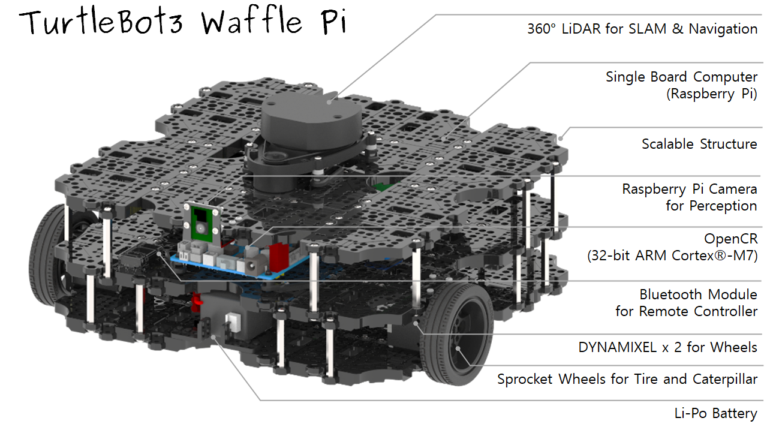
\includegraphics[width=0.8\textwidth]{Figures/turtlebot3_waffle_pi_components.png}
   \caption*{Fonte: Autoria própria.}
   \label{fig:turt2}
\end{figure}

\section{Probabilistic Roadmap}

O algoritmo Probabilistic Roadmap é um planejador de trajetória que permite que um robô se desloque de um ponto inicial a um ponto final sem a interferência de um operador evitando a colisão com obstáculos. A ideia do planejador é gerar pontos aleatórios no mapa, verificando se esses pontos são espaços livres ou não, e tentando conectar eles com os outros pontos mais próximos já gerados, caso não tenha nenhuma barreira entre esses pontos. A medida que o número de pontos cresce, vão se formando trajetórias entre todos os espaços livres do mapa, como mostrado na Figura \ref{fig:prm}.

\begin{figure} [h!]	
   \centering
   \caption{Probabilistic Roadmap}
   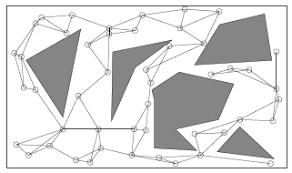
\includegraphics[width=0.6\textwidth]{Figures/images.png}
   \caption*{Fonte: Autoria própria.}
   \label{fig:prm}
\end{figure}

O algoritmo PRM tem duas fases, uma fase de construção do mapa de rotas e uma fase de questionamento. Na fase de construção, são gerados nós em pontos aleatórios do mapa que estejam em espaços livres. Cada nó desse é então ligado a número k de nós mais próximos, verificando se não a colisão no caminho. O mapa de rotas é construído então de maneira incremental e armazenado.

Na fase de questionamento, são declarados no algoritmo o ponto inicial e o ponto final do robô, sendo utilizado alguma técnica para calcular o caminho de menor custo. O algoritmo utilizado nesse caso foi o A*.

\section{Move Base}

O pacote de navegação para ROS utilizado para auxiliar nessa funcionalidade do robô é o Move Base. Através dele é possível declarar uma ação para o robô se deslocar de uma posição inicial para um posição final utilizando um planejador global e um planejador local. Nesse estudo o planejador global que será utilizado é o planejador de trajetória PRM. Na Figura \ref{fig:move} é possível ver um esquemático de como o Move Base funciona

\begin{figure} [h!]	
   \centering
   \caption{Move Base}
   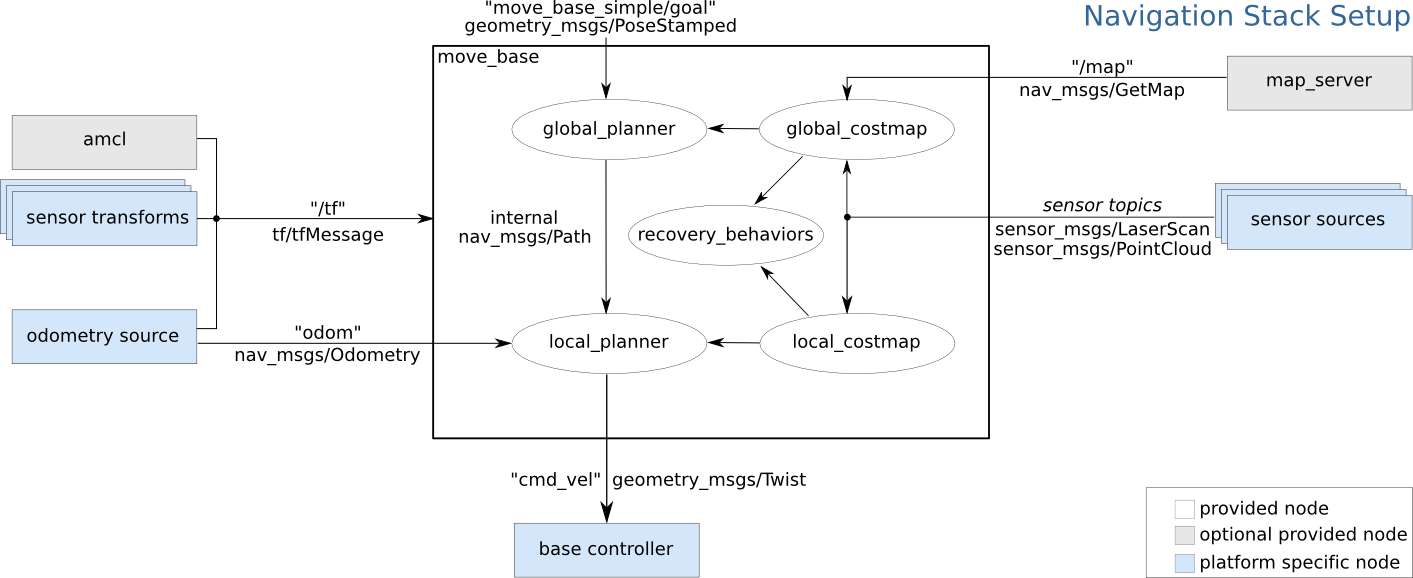
\includegraphics[width=1\textwidth]{Figures/overview_tf.png}
   \caption*{Fonte: Autoria própria.}
   \label{fig:move}
\end{figure}